\documentclass{jlreq}

\usepackage{amsmath, amssymb}
\usepackage{enumerate}
\usepackage{tikz}
\usepackage{listings, xcolor}
\usepackage{tikz}
\usetikzlibrary{shapes, positioning, arrows.meta, calc}

\renewcommand{\labelitemii}{・}

\lstset{
  basicstyle = {\ttfamily}, % 基本的なフォントスタイル 
  frame = {tbrl}, % 枠線の枠線。t: top, b: bottom, r: right, l: left
  breaklines = true, % 長い行の改行
  numbers = left, % 行番号の表示。left, right, none
  showspaces = false, % スペースの表示
  showstringspaces = false, % 文字列中のスペースの表示
  showtabs = false, % タブの表示
  keywordstyle = \color{blue}, % キーワードのスタイル。intやwhileなど
  commentstyle = {\color[HTML]{1AB91A}}, % コメントのスタイル
  identifierstyle = \color{black}, % 識別子のスタイル 関数名や変数名
  stringstyle = \color{brown}, % 文字列のスタイル
  captionpos = t % キャプションの位置 t: 上、b: 下
}

\title{情報ネットワーク応用 演習課題2A}
\author{学籍番号:1280391 \\ 細川 夏風}
\date{\today}

\begin{document}

  \maketitle
  \section{背景}
  昨今,\verb|IoT|デバイスを用いたセキュリティ事案が多く発生していることは言うまでもない.$2018$年に多く確認されたウイルス``\verb|Mirai|''は記憶に新しいだろう\cite{IPA}.\verb|IoT|デバイスはその性質上,膨大な上のやり取りがされている.必然的に乗っ取りや盗聴されると盗まれる情報の量や希少性も大きくなってくる.そのため,我々クライアントは\verb|IoT|デバイスにも多くの意識を割く必要がある.本実習ではその一例として\verb|IoT|デバイスに対して辞書攻撃のバスワードクラックを仕掛け,デバイスのカメラ機能を乗っ取るという攻撃からパスワードクラックからの対策と\verb|IoT|デバイスの脆弱性についての議論を行う.

  \section{内容}
  \subsection{環境}
  本実習の環境は以下の図の様になっている$_{\text{図}\ref{fig:environment_final_v2}}$.すでに接続している\verb|Windows|環境のサーバからサーバ内にインストールされている\verb|TeraTerm|を用いて\verb|Linux|環境の攻撃者端末に接続する.その後,複数のツールを用いて\verb|IoT|デバイスに接続する.本レポートは\verb|IoT|デバイスのパスワードを変更するまでのものとする.
  \begin{figure}[htbp]
    \centering
    \begin{tikzpicture}[
        font=\sffamily\small,
        >=Stealth,
        node distance=1.0cm, % 箱同士の基本距離
        % --- スタイル定義 ---
        envBox/.style={
            rectangle, 
            draw=black, 
            very thick, 
            fill=white,
            align=center,
            minimum width=3.2cm
        },
        envTitle/.style={
            fill=gray!30, 
            draw=black, 
            thick,
            minimum height=0.6cm, 
            minimum width=3.2cm, 
            font=\bfseries,
            anchor=south
        },
        connBox/.style={
            rectangle, 
            draw=black, 
            thick, 
            fill=white, 
            align=center, 
            minimum width=2.5cm, 
            minimum height=1.2cm,
            inner sep=2pt
        },
        arrow/.style={
            ->, 
            very thick, 
            shorten <=0pt, 
            shorten >=0pt
        }
    ]

    % === 1. 下段:Windows環境 ===
    \node[envBox, minimum height=3cm] (win) at (0,0) {
        \\[0.8cm]
        % ノートPCアイコン
        \begin{tikzpicture}[scale=0.6]
            \draw[thick, fill=white] (0,0.2) rectangle (1.2,1.0);
            \draw[thick, fill=white] (-0.2,0.2) -- (1.4,0.2) -- (1.2,0) -- (0,0) -- cycle;
        \end{tikzpicture}\\[0.5em]
        受講者用\\サーバ
    };
    % タイトルバーに名前(winTitle)を付けて、配置の基準にする
    \node[envTitle] (winTitle) at (win.north) {Windows 環境};

    % === 2. SSH接続(Windowsタイトルの「上」に配置) ===
    % winではなくwinTitleを基準にすることで、確実にタイトルから離す
    \node[connBox, above=of winTitle] (ssh) {SSH接続};

    % === 3. 上段:Linux環境(SSHの「上」に配置) ===
    \node[envBox, minimum height=3cm, above=of ssh] (lin) {
        \\[0.8cm]
        % サーバアイコン
        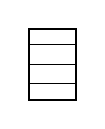
\begin{tikzpicture}[scale=0.5]
            \draw[thick, fill=white] (0,0) rectangle (1.2,1.8);
            \foreach \y in {0.4,0.9,1.4} {
                \draw (0, \y) -- (1.2, \y);
            }
        \end{tikzpicture}\\[0.5em]
        コンテンツサーバ\\攻撃者端末
    };
    \node[envTitle] (linTitle) at (lin.north) {Linux 環境};

    % === 4. ツール経由(Linuxの「右」に配置) ===
    \node[connBox, right=of lin] (tool) {ツール\\経由で\\接続};

    % === 5. IoT機器用NW(ツールの「右」に配置) ===
    \node[envBox, minimum height=4.5cm, minimum width=4cm, right=of tool] (iot) {
        \\[0.8cm]
        % IoT機器アイコン
        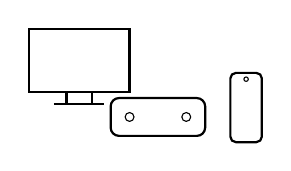
\begin{tikzpicture}[scale=0.8]
             % モニター
            \draw[thick, fill=white] (0,0.5) rectangle (1.6,1.5);
            \draw[thick, fill=white] (0.6,0.5) -- (0.6,0.3) (1.0,0.5) -- (1.0,0.3) (0.4,0.3) -- (1.2,0.3);
            % コントローラー
            \draw[thick, rounded corners=3pt] (1.3, -0.2) rectangle (2.8, 0.4);
            \draw (1.6, 0.1) circle (2pt) (2.5, 0.1) circle (2pt);
            % スマホ
            \draw[thick, rounded corners=2pt] (3.2, -0.3) rectangle (3.7, 0.8);
            \draw (3.45, 0.7) circle (1pt);
        \end{tikzpicture}\\[1em]
        IoT機器
    };
    \node[envTitle, minimum width=4cm] (iotTitle) at (iot.north) {IoT 機器用 NW};

    % === 矢印でつなぐ ===
    % 縦方向:Windowsタイトルから出発させる
    \draw[arrow] (winTitle) -- (ssh);
    \draw[arrow] (ssh) -- (lin);

    % 横方向
    \draw[arrow] (lin) -- (tool);
    \draw[arrow] (tool) -- (iot);

    \end{tikzpicture}
    \caption{演習環境の構成図}
    \label{fig:environment_final_v2}
  \end{figure}

  \newpage

  \subsection{使用ツール}
  本実習で使用するツールを以下に示す.
  \subsubsection*{Nmap}
    \verb|Nmap(|``Network Mapper''\verb|)|はネットワーク調査およびセキュリティ監査を行うためのオープンソースツールである\cite{nmap}.
    
    \verb|Nmap|の引数として,\verb|IP|アドレス($2$進数表記も可能),ホスト名が使用可能である.しかし,この際\verb|IP|アドレスと同じホスト名を引数内に$2$つ指定しても同じ結果が得られる.また,\verb|IP|アドレスは末尾にサブネットマスクを指定することによって,そのセグメント内に対してブロードキャストにポートスキャンが可能である.

    \begin{itemize}
    \item オプションの指定
      \begin{itemize}
      \item \verb|-sn|
        \begin{itemize}
          \item \verb|Ping|スキャン
          \item ホストの発見のみ実行し,結果を一覧表示する
          \item ポートスキャンは行わない        
        \end{itemize}
      \item \verb|-sL|
        \begin{itemize}
          \item \verb|List|スキャン
          \item 検査対象をリストし\verb|DNS|解決するのみで検査対象へパケットを送らない
          \item 検査対象が正しいかを確認するために用いられる
        \end{itemize}
      \item \verb|-n|
        \begin{itemize}
          \item 発見した\verb|IP|アドレスに対して\verb|DNS|の逆引きを行わない
          \item 処理高速化のために用いられる
        \end{itemize}
      \item \verb|-sS|
        \begin{itemize}
          \item \verb|TCP SYN|スキャン
          \item 対象ポートに\verb|SYN|パケットを送り,応答を確認する
          \item 実行には管理者権限が必要
        \end{itemize}
      \item \verb|-sT|
        \begin{itemize}
          \item \verb|TCP Connect|スキャン
          \item 対象ポートに接続を行い応答を確認する
          \item \verb|SYN|スキャンにクラbて,対象のホストのログに記録される可能性が高い
        \end{itemize}
      \item \verb|-A|
        \begin{itemize}
          \item \verb|OS|検知,バージョン検知,スクリプトスキャンなど,様々な処理を有効にする
          \item サービスの詳細を調査する場合に利用される
        \end{itemize}
      \item \verb|-p|
        \begin{itemize}
          \item 対象のポートを選択できる
          \item 複数選択が可能
        \end{itemize}
      \item \verb|-iL|
        \begin{itemize}
          \item 引数にファイル名をとり,そのファイル名からターゲット指定を読み込む
          \item コマンドラインで非常に巨大なホストリストを渡すのは不適切である場合が多いため,その対策として用いられる
        \end{itemize}
      \item \verb|-iR|
        \begin{itemize}
          \item インターネット上のサーバに対して無作為にポートスキャンが可能
          \item 引数にどれほどのサーバをポートスキャンするかを指定できる
        \end{itemize}
      \item \verb|--execlude|
        \begin{itemize}
          \item ホスト名を指定したあと,[]内にコンマ区切りで入力することによってスキャン対象から除外できる
        \end{itemize}
      \item \verb|--excludefile|
        \begin{itemize}
          \item 上記の\verb|--execlude|と同様の機能を提供するが,こちらはファイルに記述されたものを読み取り除外する
        \end{itemize}
      \end{itemize}
    \end{itemize}
  \subsubsection*{hydra}
  \verb|hydra|とは,並列化さらたログインクラッカーである.また,攻撃対象として多数のプロトコルをサポートしている\cite{hydra}.

  \begin{itemize}
    \item オプションの指定
      \begin{itemize}
      \item \verb|-l LOGIN| / \verb|-L FILE|
        \begin{itemize}
          \item ログイン名 (ユーザ名) を指定する
          \item \verb|LOGIN|
            \begin{itemize}
              \item 単一のログイン名を指定する場合に用いる
            \end{itemize}
          \item \verb|FILE|
            \begin{itemize}
              \item ログイン名が列挙されたファイル (リスト) を読み込む場合に用いる
            \end{itemize}
        \end{itemize}
      \item \verb|-p PASS| / \verb|-P FILE|
        \begin{itemize}
          \item パスワードを指定する
          \item \verb|PASS|
            \begin{itemize}
              \item 単一のパスワード候補を指定する場合に用いる
            \end{itemize}
          \item \verb|FILE|
            \begin{itemize}
              \item パスワード候補が列挙されたファイル (辞書ファイル) を読み込む場合に用いる
            \end{itemize}
        \end{itemize}
      \item \verb|-x MIN:MAX:CHARSET|
        \begin{itemize}
          \item 辞書ファイルを使わず, パスワードを自動生成 (ブルートフォース) して試行する
          \item \verb|MIN:MAX:CHARSET|
            \begin{itemize}
              \item \verb|最小文字数:最大文字数:文字種| の形式で指定する (例: \verb|3:5:a1| なら英小文字と数字で3~5文字)
            \end{itemize}
        \end{itemize}
      \item \verb|-e nsr|
        \begin{itemize}
          \item 辞書リスト等に加え, 特殊なパターンのパスワードを追加で試行する
          \item \verb|n|
            \begin{itemize}
              \item 空のパスワード (パスワードなし) を試行する
            \end{itemize}
          \item \verb|s|
            \begin{itemize}
              \item ログイン名と同じ文字列をパスワードとして試行する
            \end{itemize}
          \item \verb|r|
            \begin{itemize}
              \item ログイン名を逆さにした文字列をパスワードとして試行する
            \end{itemize}
        \end{itemize}
      \item \verb|-o FILE|
        \begin{itemize}
          \item 解析結果をファイルに出力する
          \item \verb|FILE|
            \begin{itemize}
              \item 発見されたログイン名とパスワードのペアを書き出すファイル名を指定する
            \end{itemize}
        \end{itemize}
      \item \verb|-t TASKS|
        \begin{itemize}
          \item 並列処理の数を指定する
          \item \verb|TASKS|
            \begin{itemize}
              \item ターゲット1台あたりの同時接続数 (スレッド数) を指定する (デフォルトは16)
            \end{itemize}
        \end{itemize}
      \item \verb|-M FILE|
        \begin{itemize}
          \item 複数のターゲットに対して攻撃を行う
          \item \verb|FILE|
            \begin{itemize}
              \item 攻撃対象のサーバ (IPアドレスやドメイン) が列挙されたファイルを指定する
            \end{itemize}
        \end{itemize}
      \item \verb|-f|
        \begin{itemize}
          \item 1つでも有効なログインペアが見つかった時点で, そのホストへの攻撃を直ちに終了する
        \end{itemize}
      \item \verb|-V|
        \begin{itemize}
          \item 詳細表示モード (Very Verbose)
          \item 試行中のログイン名とパスワードをリアルタイムで画面に表示する
        \end{itemize}
      \end{itemize}
    \end{itemize}

  \subsection{方法}
  \begin{enumerate}[(1). ]
    \item \verb|Tera Term|のホスト名に対象の\verb|IP|アドレスを入力し,他項目はデフォルトのまま\verb|OK|を押す.
    \item ユーザ\verb|ID|欄,パスワード欄に既知の\verb|ID|とパスワードを入力する.
    \item 次に,以下のコマンドから\verb|Nmap|を用いたポートスキャンを行う.
      \begin{lstlisting}
        nmap -Pn -n -A -p <IoTデバイスのIPアドレス>
      \end{lstlisting}
    \item 結果から,ポート番号$45678$に\verb|http|サービスが稼働している事がわかった.
    \item \verb|Tera Term|の機能から\verb|SSH|転送を利用し,\verb|Windows|端末から\verb|IoT|デバイスへの\verb|HTTP|通信を実現する.
    \item \verb|Tera Term|の設定から\verb|SSH|転送を押し,追加を選択する.この際,ローカルポートに$1$から$1024$でない任意のポート番号を入力する.ただし,$65535$までである.リッスンの項目は$127.0.0.1$を入力し,リモート側ホストは\verb|IoT|デバイスの\verb|IP|アドレスそ指定する.最後にポートの項目は先程\verb|HTTP|サービスの稼働を確認した$45678$である.
    \item \verb|Web|ブラウザから\verb|http://127.0.0.1:45678/|にアクセスする.アクセスすると認証画面が表示される.
    \item \verb|hydra|によって辞書攻撃を行う.このとき,ユーザ名とパスワードリストは\verb|/opt/iot/mirai/user.txt|,\verb|/opt/iot/mirai/pass.txt|内に格納されている.
      \begin{lstlisting}
        hydra –t 5 –L /opt/iot/mirai/user.txt  /opt/iot/mirai/pass.txt http-get://<IoTデバイスのIP >:45678/
      \end{lstlisting}
    \item これにより,ユーザ名\verb|admin|に対して,パスワードが\verb|88888|であることがわかった.
    \item これを使用し,\verb|FireFox|の\verb|Sign in|から管理画面へ侵入する.
    \item 管理画面に侵入したので,そこからこのユーザに対して任意の行動を取ることができる.パスワード変更もその$1$つである.
  \end{enumerate}

  \section{考察}
  今実習から以下のことが得られた.
  \begin{enumerate}[(i). ]
    \item ユーザ名を推測しやすいものにすると,パスワードクラックにかかる時間が低下する場合がある.
    \item パスワードを推測しやすいもの,何かの単語を用いると辞書攻撃の際にパスワードクラックにかかる時間が大幅に低下する事がある.
  \end{enumerate}
  
  辞書攻撃は非常に強力な攻撃の$1$つであると言える.なぜなら,パスワードやユーザ名には何かしらの単語を用いることが非常に多い.それはログインに用いる際の人為的負荷を軽減するためである.ログインの際に正規のユーザ自体も覚えられないような文字列である場合,パスワード強度としては非常に強力であるが,認証自体では適切とは言えない.その解決策として,パスワードマネージャーが多く挙げられる.\verb|Web|ブラウザ等やその他アプリケーションのログインに用いられる.これにはいくつか効果があり,単純に長く難解なパスワードを記憶する必要がなくなることがある.他にも,\verb|Web|サイトの場合,偽サイトかどうかの判断に用いることも可能だ.しかし,これにもデメリットは存在する.そのパスワードリスト自体が漏洩した場合,多くのサイトへの侵入を許してしまう.次に特定の環境に依存する場合があるということである.これはそのパスワード自体をどの媒体,どのプラットフォームに保存しているかによって環境が変化した場合,利用が単純ではないということである.しかし,それらを共有すればするほど漏洩のリスクが上昇する.そのため,他の解決策として$2$要素認証で身体情報等を用いることができればそれが最も良いが,そのようなサービスは多くない.また,最も良いとされているのは定期的にパスワードを変更することである.これらの機能や対策を総合的に用いてパスワードを作成することが現時点における最良の手段であると私は考える.

  また,今実習については攻撃対象が\verb|IoT|デバイスであることから,高負荷の攻撃を行うことが難しい.\verb|IoT|デバイスには多くの制約がつきまとう.計算能力もその$1$つである.そのため,多くの場合に用いられるのがソーシャルエンジニアリングである.計算機の特定の機能を悪用すること無く対象に攻撃を行うことである.これによって計算機に依存せず攻撃を行うことができる.

  最後に\verb|IoT|デバイスに侵入されることのデメリットについて議論を行う.私が考える\verb|IoT|デバイスがクラックされることの最大のデメリットはその\verb|IoT|デバイスが接続されているネットワークについての情報が攻撃者に把握される可能性があることであると考える.些細な\verb|IoT|デバイスからその上位ネットワークについて,それに接続される可能性さえ孕んでいる.もちろんこれは稀なケースであることには変わりない.しかし,いくつか事例は存在する.ロジテック製のルータに存在した脆弱性を用いて,外部から操作され攻撃の拠点として使われた事例もその$1$つである.これに対する対策は\verb|VLAN|での隔離という方法が取られることが多い.他にも根本的に孤立したデバイス(\verb|IoT|デバイスや\verb|Web|カメラなど)のセキュリティを強化することや内部ネットワークに直接アクセスできないようにすることなどが挙げられる.最終的に必要なのはどのデバイスにも簡単にアクセスさせないこと,もしアクセスがある場合はその部分のみ\verb|VLAN|等で切り離すことである.そして,ソーシャルエンジニアリングに対する理解を深め自身が攻撃を受けたことを理解し,それに対する適切な処置を取れるようになる必要がある.

  こうした,\verb|IoT|デバイスの乗っ取りや盗聴はこれから\verb|IoT|デバイスが増えていく中で増加していくだろう.そのため,それらを利用する立場に置かれる私たちがこの問題を理解し,対処することができるようになることがこの実習での意義の最たるものである考える.更にはこの問題が世に周知され,多くの被害が緩和されることを期待し本報告の結びとする.

\begin{thebibliography}{99}
  \bibitem{IPA} 情報セキュリティ白書2019,独立行政法人情報処理推進機構(IPA),2019年8月8日
  \bibitem{nmap} \verb|Nmap|公式ページ,\verb|https://nmap.org/|
  \bibitem{hydra} \verb|Kali Linux Tools|,\verb|https://www.kali.org/tools/hydra/|
\end{thebibliography}
\end{document}
